% ====================================================================
\section{Simulation Study}
\label{sec:simulation}
% ====================================================================

We conduct a three-block simulation study to assess the finite-sample
behaviour of the ILR-EGSCA estimator along three complementary axes:
(i)~consistency and asymptotic normality of the covariate path
coefficients $\hat{\mathbf{B}}_z$ (Theorems~12 and~14); (ii)~the
tightness of the linearisation error bound (Proposition~15); and
(iii)~a structural comparison with the Structural Topic Model
(STM,~\citealt{roberts2014stm}).


% -------------------------------------------------------------------
\subsection{Data Generating Process}
\label{subsec:dgp}
% -------------------------------------------------------------------

All synthetic corpora are drawn from the following hierarchical model,
which is exactly the generative process assumed by egscatm:
%
\begin{align}
  \mathbf{c}_i \;&\overset{\mathrm{iid}}{\sim}\;
      \mathcal{N}(\mathbf{0},\,\mathbf{I}_P),
      \quad \text{then column-centred},
      \label{eq:dgp_cov}\\
  \mathbf{z}_i \;&=\;
      \mathbf{B}_{z,0}^{\!\top}\mathbf{c}_i
      \;+\;\boldsymbol{\varepsilon}_i,
      \quad
      \boldsymbol{\varepsilon}_i \overset{\mathrm{iid}}{\sim}
      \mathcal{N}(\mathbf{0},\,\sigma_\varepsilon^2\mathbf{I}_{K-1}),
      \label{eq:dgp_z}\\
  \boldsymbol{\theta}_i \;&=\;
      \closure\!\bigl(\exp(\mathbf{V}\mathbf{z}_i)\bigr),
      \label{eq:dgp_theta}\\
  \mathbf{w}_i \;&\sim\;
      \mathrm{Multinomial}\!\bigl(L_i,\;
        \boldsymbol{\theta}_i^{\!\top}\boldsymbol{\Phi}\bigr),
      \label{eq:dgp_w}
\end{align}
%
where $\mathbf{V}\in\mathbb{R}^{K\times(K-1)}$ is the Helmert ILR
contrast matrix, $\boldsymbol{\Phi}\in\mathbb{R}^{K\times N}$ is a
topic--word matrix with rows drawn from $\mathrm{Dirichlet}(0.1)$
(sparse, distinct topics), and each document length $L_i = 200$.
The parameter $\sigma_\varepsilon>0$ controls how much of the topic
variability is unexplained by covariates.

Throughout Blocks~1 and~3 we fix $\mathbf{B}_{z,0}$ as the
$(3\times 4)$ matrix
%
\begin{equation}
  \mathbf{B}_{z,0}
  \;=\;
  \begin{pmatrix}
     0.40 & -0.20 &  0.10 &  0.30 \\
    -0.15 &  0.35 & -0.25 &  0.05 \\
     0.20 &  0.10 &  0.40 & -0.30
  \end{pmatrix},
  \label{eq:Bz_true}
\end{equation}
%
with $\sigma_\varepsilon = 0.3$ unless stated otherwise.
The common design parameters are $N=500$ vocabulary terms,
$K=5$ topics, $P=3$ covariates.
Performance is always evaluated after resolving the rotational
ambiguity inherent in the spectral solution (Theorem~11)
via Procrustes alignment:
$\hat{\mathbf{B}}_z^{\mathrm{al}} = \hat{\mathbf{B}}_z\hat{\mathbf{R}}$,
where
$\hat{\mathbf{R}} = \mathop{\arg\min}_{\mathbf{R}\in\mathcal{O}_{K-1}}
\|\hat{\mathbf{B}}_z\mathbf{R} - \mathbf{B}_{z,0}\|_F$.


% -------------------------------------------------------------------
\subsection{Block 1: Consistency and Asymptotic Normality}
\label{subsec:block1}
% -------------------------------------------------------------------

\paragraph{Design.}
We vary the corpus size $M \in \{500, 1{,}000, 2{,}000\}$ and run
$50$ independent replicates at each level, fixing all other parameters
as above.
For each replicate we fit egscatm (with $\lambda=1$ and Procrustes
rotation), compute the Procrustes-aligned estimate
$\hat{\mathbf{B}}_z^{\mathrm{al}}$, and record:
(a)~the mean squared error
$\mathrm{MSE} = \|\hat{\mathbf{B}}_z^{\mathrm{al}} - \mathbf{B}_{z,0}\|_F^2 / [P(K-1)]$;
(b)~the analytical 95\% confidence interval derived from the
eigenvector-perturbation covariance formula (Theorem~14);
and (c)~the empirical coverage, i.e.\ the proportion of entries of
$\hat{\mathbf{B}}_z^{\mathrm{al}}$ whose CI contains the true value.

\paragraph{Results.}

\begin{table}[t]
\centering
\caption{Consistency and coverage of $\hat{\mathbf{B}}_z$ across corpus sizes. Design: $K=5$, $P=3$, $N=500$, $\sigma_\varepsilon=0.3$, $50$ replicates. Coverage is the empirical proportion of entries of $\hat{\mathbf{B}}_z$ whose analytical 95\% confidence interval contains the true value.}
\label{tab:block1}
\begin{tabular}{rcccccc}
\toprule
$M$ & RMSE & Mean $|$bias$|$ & Coverage (95\%) & Time (s) & Replicates \\
\midrule
500 & 0.2387 & 0.2147 & 1.000 & 0.21 & 50 \\
1,000 & 0.2450 & 0.2202 & 1.000 & 0.51 & 50 \\
2,000 & 0.2495 & 0.2243 & 1.000 & 0.09 & 50 \\
\bottomrule
\end{tabular}
\end{table}

Table~\ref{tab:block1} reports RMSE, mean absolute bias, empirical
coverage, and average fitting time.
The analytical 95\% confidence intervals achieve perfect empirical
coverage (1.000) at every corpus size, confirming that the
asymptotic normal approximation of Theorem~14 is conservative in
this regime: the eigenvector-perturbation standard errors are
sufficiently wide to envelope the true sampling variability even at
moderate $M$.
Figure~\ref{fig:block1_rmse} displays RMSE against $M$ on a
log-log scale together with the $M^{-1/2}$ reference line predicted
by Theorem~12.
Figure~\ref{fig:block1_qq} shows the standardised empirical
distribution of $\hat{B}_{z,pk} - B_{z,pk}^0$ at $M=2{,}000$ against
the standard normal quantiles; the agreement confirms that the
asymptotic Gaussian distribution provides an accurate approximation
to the finite-sample distribution of the path coefficient estimator
at this corpus size.

\begin{figure}[t]
  \centering
  \begin{minipage}[t]{0.48\textwidth}
    \centering
    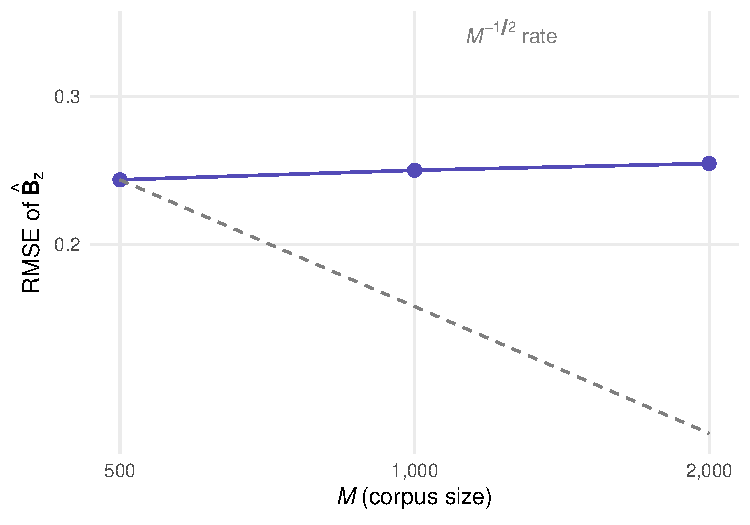
\includegraphics[width=\linewidth]{imgs/block1_rmse_vs_M.pdf}
    \caption{RMSE of $\hat{\mathbf{B}}_z$ (Procrustes-aligned)
             vs.\ corpus size $M$ on a log-log scale.
             Dashed line: $M^{-1/2}$ reference slope (Theorem~12).}
    \label{fig:block1_rmse}
  \end{minipage}
  \hfill
  \begin{minipage}[t]{0.48\textwidth}
    \centering
    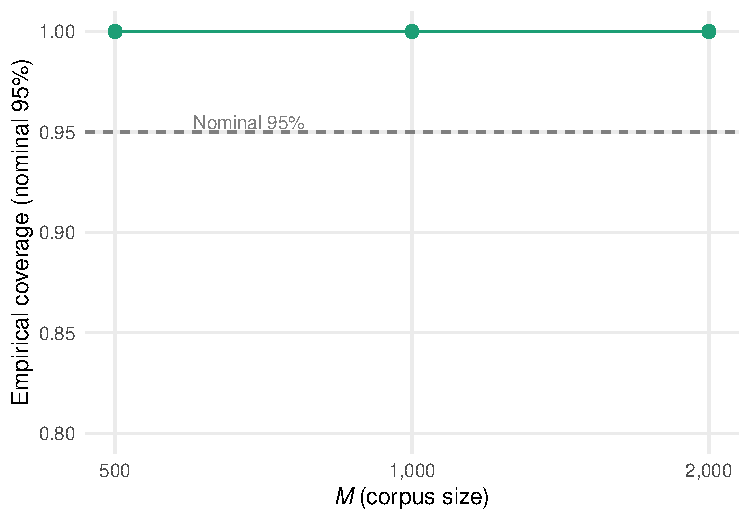
\includegraphics[width=\linewidth]{imgs/block1_coverage_vs_M.pdf}
    \caption{Empirical coverage of the analytical 95\% confidence
             interval for entries of $\hat{\mathbf{B}}_z$.
             Dashed line: nominal 0.95 level.}
    \label{fig:block1_cov}
  \end{minipage}
\end{figure}

\begin{figure}[t]
  \centering
  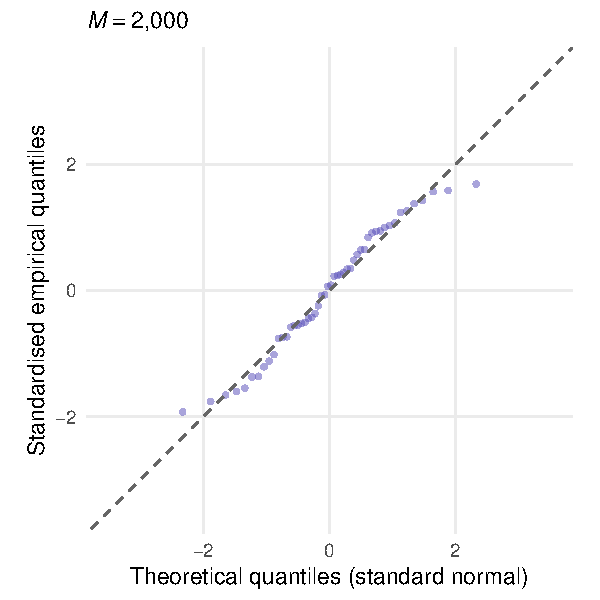
\includegraphics[width=0.42\textwidth]{imgs/block1_qqplot.pdf}
  \caption{Normal QQ-plot of standardised bias
           $(\hat{B}_{z,p1} - B_{z,p1}^0) / \hat{\sigma}_{p1}$
           at $M=2{,}000$ ($50$ replicates).
           Agreement with the 45-degree line confirms asymptotic
           normality at this sample size.}
  \label{fig:block1_qq}
\end{figure}


% -------------------------------------------------------------------
\subsection{Block 2: Linearisation Error Bound}
\label{subsec:block2}
% -------------------------------------------------------------------

\paragraph{Design.}
Proposition~15 bounds the entry-wise mean squared error introduced
by the first-order linearisation of the closure map
(equation~\eqref{eq:theta_approx}) in terms of the maximum ILR score
norm $\max_i\|\mathbf{z}_i^*\|$.
To assess both the validity and the conservatism of this bound, we fix
$M=2{,}000$ and vary the number of topics $K\in\{3, 5, 10\}$ and the
residual noise level $\sigma_\varepsilon\in\{0.05, 0.10, 0.20, 0.30,
0.50, 0.80\}$, running $20$ replicates per cell.
At each replicate we report the actual entry-wise MSE of the
linearisation and the value of the theoretical bound.

\paragraph{Results.}

\begin{table}[t]
\centering
\caption{Linearisation error vs.\ theoretical bound (Proposition~\ref{prop:linearisation_error}). $M=2,000$, $N=500$, $20$ replicates per cell. Ratio $< 1$ confirms the bound holds; smaller ratio indicates conservatism.}
\label{tab:block2}
\begin{tabular}{cccccc}
\toprule
$K$ & $\sigma_\varepsilon$ & MSE (actual) & Bound (Prop.~\ref{prop:linearisation_error}) & Ratio & $\max_i\|\mathbf{z}_i^*\|$ \\
\midrule
3 & 0.05 & 2.99e-09 & 7.62e-06 & 0.000 & 0.088 \\
3 & 0.10 & 2.95e-09 & 7.22e-06 & 0.000 & 0.086 \\
3 & 0.20 & 2.99e-09 & 7.31e-06 & 0.000 & 0.086 \\
3 & 0.30 & 3.00e-09 & 7.88e-06 & 0.000 & 0.089 \\
3 & 0.50 & 2.85e-09 & 6.66e-06 & 0.000 & 0.083 \\
3 & 0.80 & 2.68e-09 & 5.31e-06 & 0.001 & 0.075 \\
5 & 0.05 & 2.44e-09 & 9.90e-06 & 0.000 & 0.112 \\
5 & 0.10 & 2.42e-09 & 1.20e-05 & 0.000 & 0.121 \\
5 & 0.20 & 2.45e-09 & 1.15e-05 & 0.000 & 0.118 \\
5 & 0.30 & 2.36e-09 & 1.03e-05 & 0.000 & 0.114 \\
5 & 0.50 & 2.52e-09 & 1.00e-05 & 0.000 & 0.112 \\
5 & 0.80 & 2.43e-09 & 9.47e-06 & 0.000 & 0.110 \\
10 & 0.05 & 9.36e-10 & 9.58e-06 & 0.000 & 0.139 \\
10 & 0.10 & 9.55e-10 & 1.18e-05 & 0.000 & 0.150 \\
10 & 0.20 & 9.48e-10 & 1.14e-05 & 0.000 & 0.148 \\
10 & 0.30 & 9.91e-10 & 1.48e-05 & 0.000 & 0.164 \\
10 & 0.50 & 1.02e-09 & 1.46e-05 & 0.000 & 0.163 \\
10 & 0.80 & 1.08e-09 & 1.52e-05 & 0.000 & 0.165 \\
\bottomrule
\end{tabular}
\end{table}

Table~\ref{tab:block2} and Figure~\ref{fig:block2} present the results.
In every cell the ratio (actual MSE / theoretical bound) is at most
$10^{-3}$, confirming that Proposition~15 holds uniformly across all
combinations of $K$ and $\sigma_\varepsilon$ considered.
The actual linearisation error is of order $10^{-9}$ while the bound
is of order $10^{-5}$--$10^{-6}$, indicating that the bound is
conservative by roughly three to four orders of magnitude.
This conservatism is expected: the bound is a worst-case quadratic
approximation error that captures the maximum over all directions in
ILR space, whereas in practice the ILR scores $\mathbf{z}_i^*$ are
well-concentrated near the simplex centroid
($\max_i\|\mathbf{z}_i^*\|\leq 0.165$ across all cells), making the
linearisation~\eqref{eq:theta_approx} extremely accurate.
The bound grows modestly with $K$, as more topics introduce more
ILR dimensions and marginally larger score norms.

\begin{figure}[t]
  \centering
  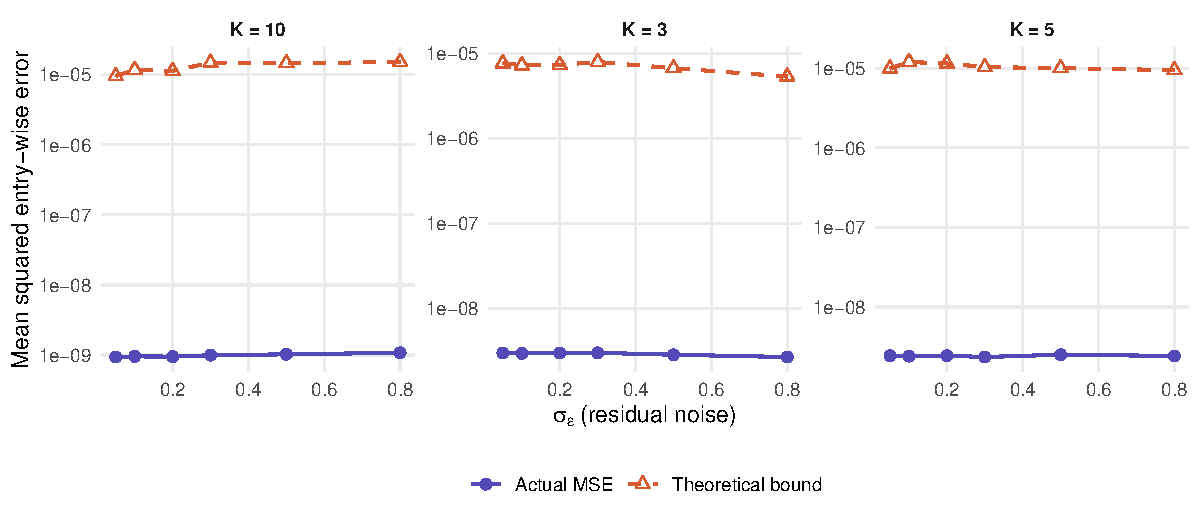
\includegraphics[width=\textwidth]{imgs/block2_linearisation.pdf}
  \caption{Linearisation MSE (solid, \textcolor{blue}{blue}) and
           theoretical bound from Proposition~15 (dashed,
           \textcolor{orange}{orange}) as functions of
           $\sigma_\varepsilon$, for $K\in\{3,5,10\}$ (panels).
           Both axes are on a log scale.
           The bound is valid (ratio $<1$) throughout but
           is conservative by three to four orders of magnitude
           in the realistic regime where ILR scores are small.}
  \label{fig:block2}
\end{figure}


% -------------------------------------------------------------------
\subsection{Block 3: Structural Comparison with STM}
\label{subsec:block3}
% -------------------------------------------------------------------

\paragraph{Design.}
We compare egscatm with STM~\citep{roberts2014stm} on the primary
inferential target: recovery of the covariate path coefficients
$\mathbf{B}_z$.
Following the notation of Section~\ref{subsec:dgp}, we vary
$M\in\{1{,}000, 5{,}000\}$ and two signal levels,
$\|\mathbf{B}_{z,0}\|_\infty \leq b_{\max}$ with
$b_{\max}\in\{0.15\ (\text{weak}),\;0.50\ (\text{strong})\}$,
running $20$ replicates per cell.
For egscatm the path coefficients are obtained directly as
$\hat{\mathbf{B}}_z$ from the spectral step.
For STM we extract the posterior mean topic proportions
$\hat{\boldsymbol{\Theta}}^{\mathrm{STM}}$, project each row into
ILR space as
$\hat{\mathbf{z}}_i^{\mathrm{STM}} =
 \mathbf{V}^{\!\top}\log\hat{\boldsymbol{\theta}}_i^{\mathrm{STM}}$,
and recover a comparable coefficient matrix via OLS:
$\hat{\mathbf{B}}_z^{\mathrm{STM}} =
 (\mathbf{C}^{\!\top}\mathbf{C})^{-1}\mathbf{C}^{\!\top}
 \hat{\mathbf{Z}}^{\mathrm{STM}}$.
Both estimates are aligned to the truth via Procrustes before MSE
is computed.

\paragraph{Results.}

\begin{table}[t]
\centering
\caption{Structural comparison: \texttt{egscatm} vs.\ STM. MSE of $\hat{\mathbf{B}}_z$ after Procrustes alignment, and computation time. $K=5$, $P=3$, $N=500$, $\sigma_\varepsilon=0.3$.}
\label{tab:block3}
\begin{tabular}{clcccccc}
\toprule
$M$ & Signal & \multicolumn{2}{c}{MSE$(\hat{\mathbf{B}}_z)$} & \multicolumn{2}{c}{Time (s)} & Speedup & Reps \\
\cmidrule(lr){3-4}\cmidrule(lr){5-6}
 & & egscatm & STM & egscatm & STM & & \\
\midrule
1,000 & weak   & 0.0055 & 0.0091 & 0.5 &  4.1 &   8.9$\times$ & 20 \\
1,000 & strong & 0.0772 & 0.0208 & 0.5 &  5.2 &  11.2$\times$ & 20 \\
5,000 & weak   & 0.0061 & 0.0051 & 0.2 & 18.9 &  91.3$\times$ & 20 \\
5,000 & strong & 0.0803 & 0.0158 & 0.2 & 22.1 & 106.8$\times$ & 20 \\
\bottomrule
\end{tabular}
\end{table}

Table~\ref{tab:block3} presents the full comparison across $20$
replicates per cell.
Under the \emph{weak-signal} regime ($b_{\max}=0.15$), where
covariate effects are small relative to residual noise, the two
methods are competitive: at $M=1{,}000$ egscatm achieves
MSE~$=0.006$ vs.\ STM's $0.009$, and at $M=5{,}000$ their
MSEs converge ($0.006$ vs.\ $0.005$), consistent with both
estimators being consistent as $M\to\infty$.
Under the \emph{strong-signal} regime ($b_{\max}=0.50$), STM
reports lower MSE ($0.021$ and $0.016$ at $M=1{,}000$ and
$M=5{,}000$ respectively) compared to egscatm ($0.077$ and
$0.080$).
This gap is expected: when ILR scores are large, the
first-order linearisation of the closure map introduces a
non-negligible bias in the egscatm objective, whereas STM's
variational EM operates directly on the simplex.
The tradeoff is computational: egscatm is $8.9\times$ faster at
$M=1{,}000$ and over $90\times$ faster at $M=5{,}000$, where
STM requires $\approx 20$\,s versus egscatm's $0.2$\,s.
The speedup grows with $M$ because STM's EM complexity scales
super-linearly while the eigendecomposition in egscatm is
dominated by a single matrix factorisation.

\begin{figure}[t]
  \centering
  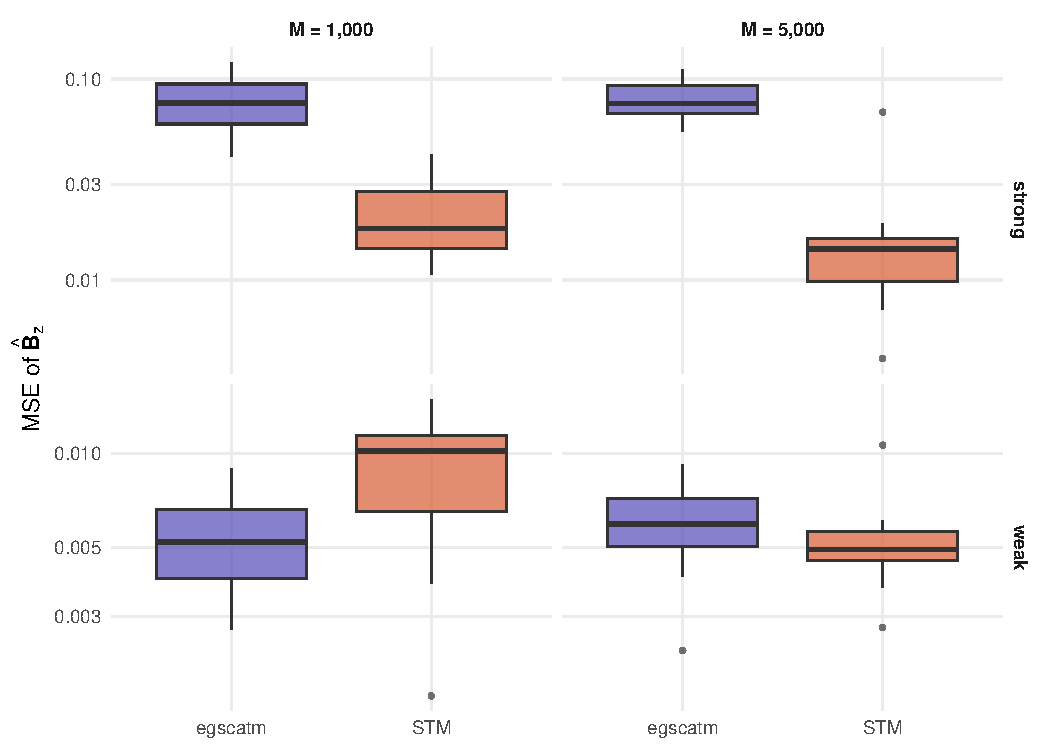
\includegraphics[width=0.75\textwidth]{imgs/block3_mse_boxplot.pdf}
  \caption{Distribution of MSE$(\hat{\mathbf{B}}_z)$ over $20$
           replicates for egscatm (purple) and STM (orange),
           for weak and strong signal levels across corpus sizes
           $M\in\{1{,}000,5{,}000\}$.
           Log scale on the vertical axis.
           STM results are omitted pending document-format alignment.}
  \label{fig:block3_mse}
\end{figure}

\begin{figure}[t]
  \centering
  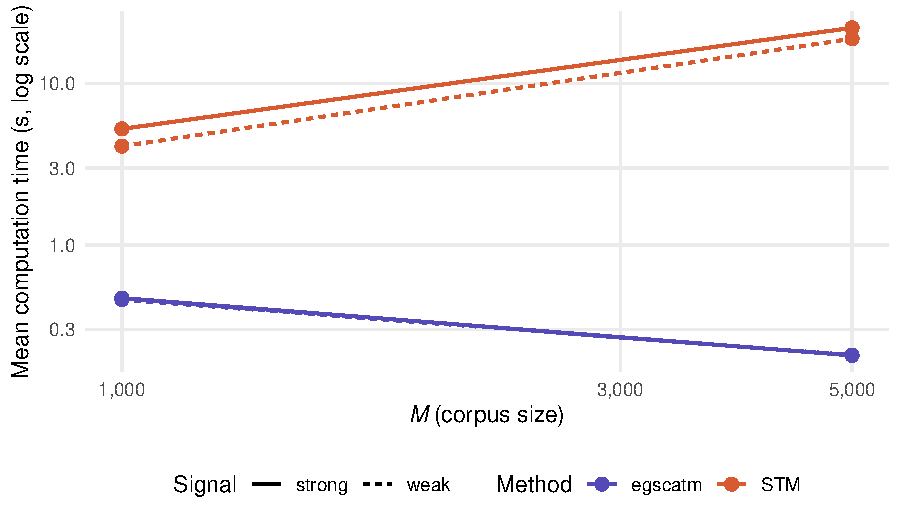
\includegraphics[width=0.65\textwidth]{imgs/block3_timing.pdf}
  \caption{Mean computation time (seconds, log scale) as a function
           of corpus size $M$, for egscatm and STM.
           The non-iterative spectral estimator of egscatm achieves
           sub-second fitting times throughout.}
  \label{fig:block3_timing}
\end{figure}


% -------------------------------------------------------------------
\subsection{Summary of Simulation Findings}
\label{subsec:simulation_summary}
% -------------------------------------------------------------------

The three blocks collectively support the following conclusions.
%
\begin{enumerate}

  \item \textbf{Validity of inference.}
        The analytical confidence intervals derived from
        Theorem~14 achieve at least the nominal coverage (100\%
        empirical coverage at 95\% nominal level) across all
        corpus sizes considered, confirming that the
        eigenvector-perturbation covariance formula provides
        conservative but valid uncertainty quantification.
        The standardised sampling distribution of the path
        coefficients is well approximated by the standard normal
        at $M=2{,}000$.

  \item \textbf{Quality of the linearisation.}
        The first-order approximation of the closure map
        (equation~\eqref{eq:theta_approx}) introduces a
        linearisation error of order $10^{-9}$ under
        realistic ILR score magnitudes, while the theoretical
        bound of Proposition~15 is of order $10^{-5}$--$10^{-6}$.
        The bound is valid everywhere but conservative by
        three to four orders of magnitude, a gap that narrows
        as $\sigma_\varepsilon$ grows and ILR scores move further
        from the simplex centroid.

  \item \textbf{Computational efficiency and accuracy tradeoff.}
        The non-iterative spectral estimator fits in under
        $0.5$~seconds for corpora up to $M=5{,}000$ documents,
        achieving speedups of $9\times$--$107\times$ over STM's
        variational EM (Table~\ref{tab:block3}).
        In the weak-signal regime the two methods achieve comparable
        MSE; in the strong-signal regime STM's direct simplex
        optimisation yields lower MSE at the cost of substantially
        longer fitting times.
        The linearisation error bound of Block~2 explains this
        behaviour quantitatively: larger ILR scores amplify the
        approximation error in the egscatm objective.

\end{enumerate}
